\documentclass[a4paper,openright,11pt]{report}

%
% Times New Roman font.
%
\usefont{T1}{ptm}{m}{n}
\selectfont


% Packages a utilizar e respetivos parâmetros.
\usepackage{indentfirst}
\usepackage{inputenc}
\usepackage{enumitem}
\usepackage[portuguese]{babel}
\usepackage{graphicx}
\usepackage{float}
\usepackage{url}

\makeatletter
\let\NAT@parse\undefined
\makeatother
\usepackage{hyperref}

\addto{\captionsenglish}{\renewcommand{\bibname}{References}}
% Definições das dimensões das páginas
\setlength{\textheight}{24.00cm}
\setlength{\textwidth}{15.50cm}
\setlength{\topmargin}{0.35cm}
\setlength{\headheight}{0cm}
\setlength{\headsep}{0cm}
\setlength{\oddsidemargin}{0.25cm}
\setlength{\evensidemargin}{0.25cm}

%
% Times New Roman font.
%
\usefont{T1}{ptm}{m}{n}
\selectfont

%
%title
%
\title{%
  \vspace{-55mm}
  \begin{minipage}[l]{150mm}
    \resizebox{50mm}{!}{
\includegraphics{./figures/logo_isel.png}}
  \end{minipage}\\
  \vspace{20mm}
  \bfseries{Corporate Collaboration \par Relatório de Progresso}
}

%
%authors
%
\author{%
  \begin{tabular}{lll}
      & David Fidalgo \\
      & goncalo9marco@hotmail.com\\
      & 968 225 962 \\
      & 45365 \\
  \\
    & Pedro Santos \\
    & santos.pedroc@gmail.com \\
    & 962 942 930 \\
    & 45366 \\
  \\
    & Valdemar Antunes \\
    & ValdemarPCA@hotmail.com \\
    & 966 439 259 \\
    & 44865 
  \end{tabular}
} 

%
% date
%
\date{%
\vspace{30mm}
\begin{center}
  \begin{tabular}{ccc}
    & {Orientadores:} \\
    & Paula Graça, ISEL, paula.graca@isel.pt \\
    & Diogo Pacheco, Do iT Lean, diogo.pacheco@doitlean.com\\
  \end{tabular}\\
\end{center}
\vspace{20mm}
Relatório de progresso realizado no âmbito de Projecto e Seminário,\\
do curso de licenciatura em Engenharia Informática e de Computadores\\
Semestre de Verão 2019/2020
\vspace{10mm}\\
4 de Maio de 2020}

\begin{document}
\thispagestyle{empty}
\maketitle

\tableofcontents{}

\addcontentsline{toc}{section}{Introdução}
\section*{Introdução}\label{sec:intro}

\addcontentsline{toc}{subsection}{Enquadramento}
\subsection*{Enquadramento}
O mercado de hoje, cada vez mais tecnológico, exigente e desafiador, impõe um ritmo às empresas que, para
além de gerirem os seus principais processos de negócio, estas têm também uma dinâmica significativa de
atividades internas para as ajudar no seu crescimento e competitividade. Em particular, as empresas do setor
das tecnologias de informação, mantêm atividades internas tais como participação em feiras de emprego,
partilha de conhecimento através de apresentações informais, desenvolvimento de componentes de software,
ofertas de formação, atividades lúdicas, entre muitas outras. Para isso, tem que existir uma coordenação de
recursos que nem sempre é fácil, dada a sua alocação aos projetos em curso. Contudo, se existir um
planeamento atempado gerido através de uma plataforma de colaboração, o processo pode ser agilizado,
permitindo não só o registo e divulgação das necessidades internas, bem como a aceitação de candidaturas por
parte dos colaboradores mais interessados na sua realização.

\addcontentsline{toc}{subsection}{Objetivos}
\subsection*{Objetivos}
A aplicação proposta visa a implementação de uma plataforma colaborativa para agilizar a resposta a necessidades internas das empresas, nomeadamente a
organização de eventos, partilha de conhecimento, ofertas formativas, entre outras. 

\addcontentsline{toc}{section}{Formulação do problema}
\section*{Formulação do Problema}

\addcontentsline{toc}{subsection}{Estado da Arte}
\subsection*{Estado da Arte}
As plataformas de colaboração existentes no mercado atual apresentam um elevado nível de complexidade, incluindo ferramentas como calendários partilhados, partilha de ficheiros, mensagens instantâneas, armazenamento na \textit{cloud}, video-conferência, entre outros. A aplicação desenvolvida neste âmbito não procura igualar todas as funcionalidades das plataformas já existentes, mas sim agilizar a dinâmica de atividades internas que ocorrem diariamente nas empresas. Visa essencialmente facilitar a procura de pessoas para cumprir certas necessidades que existam no âmbito das atividades internas da empresa.

\addcontentsline{toc}{section}{Implementação}
\section*{Implementação}

\addcontentsline{toc}{subsection}{Visualização de necessidades}
\subsection*{Visualização de necessidades}\label{sec:necessities}

O utilizador ao carregar no botão \textit{Necessities} presente na barra da aplicação, será redirecionado para o ecrã responsável pela apresentação das necessidades. 
O intuito do mesmo consiste na apresentação das necessidades criadas pela comunidade empresarial, sendo possível aplicar filtros e/ou pesquisar pelo título de uma necessidade de modo a que sejam apresentadas apenas as necessidades alvo.
As necessidades são apresentadas num \textit{widget} tabela, cujas colunas apresentam informação relevante como título, categoria, prioridade, localização e o número de participantes até ao momento. Sempre que o utilizador pretender criar uma nova necessidade, apenas tem que carregar no botão \textit{Create Necessity} e será redirecionado para um novo ecrã, onde poderá completar a criação.
A seleção do título de uma necessidade promove a navegação para o ecrã dos detalhes da mesma. Se se verificar que o utilizador é o autor de uma das necessidades poderá editá-la carregando no ícone que aparece na ultima coluna, da linha em questão, da tabela.
A barra de pesquisa permite que o utilizador procure uma necessidade pelo seu título.
Os filtros aplicáveis são apresentados em três \textit{widgets} distintos. Dois \textit{dropdowns}, um para permitir a escolha de qual a prioridade e outro para distinguir entre necessidades no exterior e no interior das instalações da empresa.
É ainda apresentado um \textit{widget} tabela, de uma só coluna, que permite a seleção das categorias a que as necessidades pertencem, selecionando uma \textit{checkbox}.  
Sempre que exista uma mudança na seleção que algum dos \textit{widgets} de filtragem de necessidades ou uma introdução de texto na barra de pesquisa, a tabela é atualizada para apresentar apenas aquelas que verifiquem as características alvo. 

\addcontentsline{toc}{subsection}{Visualização de necessidades num calendário}
\subsection*{Visualização de necessidades num calendário}\label{sec:calendarNecessitiesView}
O utilizador ao carregar no botão \textit{Calendar} presente na barra da aplicação, será redirecionado para o ecrã responsável por mostrar num calendário, todas as necessidades existentes, organizadas por datas. 
O objetivo deste ecrã é apresentar de uma forma mais organizada e estruturada, todas as necessidades criadas pela empresa, sendo possível filtrar por entre elas. 
Para preencher o calendário, para cada necessidade, é criado um objeto \textit{Event} com a sua informação. 
Cada evento estará representado no calendário com uma cor diferente de forma a fazer uma distinção entre, necessidades criadas pelo utilizador autenticado, necessidades associadas de alguma forma com o utilizador autenticado, nomeadamente uma inscrição, e necessidades criadas por outros utlizadores.
Se o utilizador carregar num evento, este é redirecionado para o seu ecrã de detalhe. 
É possível filtrar eventos pela sua categoria, através de um popover menu contém todas as categorias existentes. 
Caso seja selecionada uma categoria, são removidos todos os eventos presentes no calendário, e de seguida, renderizado com os novos eventos filtrados.

\addcontentsline{toc}{subsection}{Criação e edição de necessidades}
\subsection*{Criação e edição de necessidades}\label{sec:necessityCreation}

O utilizador irá ser redirecionado para este ecrã sempre que tenha a intenção de criar ou alterar uma necessidade.
A funcionalidade deste ecrã é criar necessidades ou alterar necessidades existentes.
Quando um utilizador clica no botão \textit{Create Necessity}, virá para este ecrã com o intuito de criar uma necessidade.
Neste caso, o ecrã apresentará os vários campos necessários para a criação desta.
Se o utilizador desejar editar uma necessidade, primeiramente, só o poderá fazer se for o autor desta.
Neste caso, o ecrã apresentará os campos já preenchidos com os dados atuais da necessidade e a possibilidade de os alterar livremente.

Os botões presentes neste ecrã são apenas dois:
\begin{enumerate}
    \item \textit{Cancel} --- aprensenta um \textit{pop-up} a pedir a confirmação do utilizador, após confirmação a criação ou edição será cancelada e o utilizador redirecionado para o ecrã onde estava anteriormente.
    \item \textit{Save} --- guarda as alterações a efetuar na necessidade e cria uma ligação ao servidor para modificar a base de dados com uma nova necessidade ou alterando uma necessidade pré-existente.
\end{enumerate}

\addcontentsline{toc}{section}{Modelo EA}
\section*{Modelo EA}\label{sec:db}

\begin{figure}[H]
  \centering 
  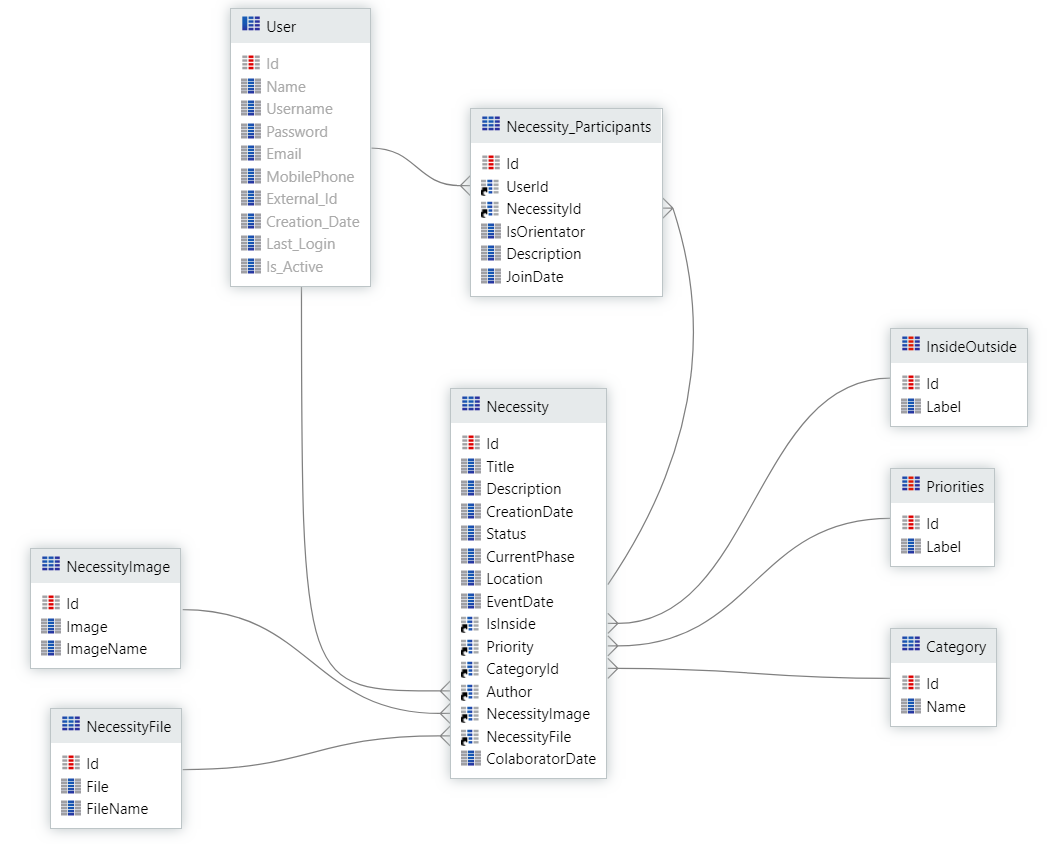
\includegraphics[scale=0.4]{figures/DataModel.png}
  \caption{Modelo de dados}\label{fig:datamodel}
\end{figure}

\addcontentsline{toc}{subsection}{Modelo de dados}
\subsection*{Modelo de Dados}\label{subsec:ModeloDados}
O conceito predominante no modelo de dados, (\ref{fig:datamodel}), é o de necessidade, representado pela tabela \textit{Necessity}. 
Uma necessidade é caracterizada por diversos elementos dos quais destacamos o \textit{Status} que corresponde ao estado da mesma, 
podendo ter por exemplo os valores \"Arquivado\" ou \"A Decorrer\", a \textit{CurrentPhase} que indica a fase de candidaturas atual, 
podendo ser para orientadores ou participantes, e ainda a \textit{ColaboratorDate} que representa a data limite das candidaturas 
à posição de orientador. 
As tabelas \textit{NecessityImage} e \textit{NecessityFile} existem para o propósito de guardar ficheiros, 
aliviando a quantidade de dados guardada em cada tuplo \textit{Necessity}, 
seguindo também as boas práticas da plataforma \textit{OutSystems}. 
A entidade \textit{InsideOutside} serve para representar a localização das necessidades relativamente a serem 
dentro das instalações da empresa ou fora. A mesma, juntamente com a entidade \textit{Priorities} 
são entidades estáticas cuja funcionalidade é manter dados persistentes na base de dados.
Com o objetivo de guardar informação de candidaturas a necessidades, é definida a entidade \texttt{\textit{Necessities\char`_Participants}} que 
contempla o identificador da mesma, o identificador do utilizador, a descrição associada à candidatura, 
se esta candidatura é para posição de orientador ou de participante e a data da candidatura. 
Um utilizador pode ser um participante, um autor ou um orientador da necessidade. 
Este poderá ainda ter o cargo de administrador, cujos privilégios incluem editar as categorias representadas pela 
entidade \textit{Category}.

\addcontentsline{toc}{subsection}{4 \textit{Layer Canvas}}
\subsection*{4 Layer Canvas}\label{sec:4lc}

Para desenharmos a arquitetura da nossa solução, seguimos a metodologia da plataforma \textit{OutSystems}, a \textit{4 Layer Canvas}.

\begin{figure}[h]
  \centering 
  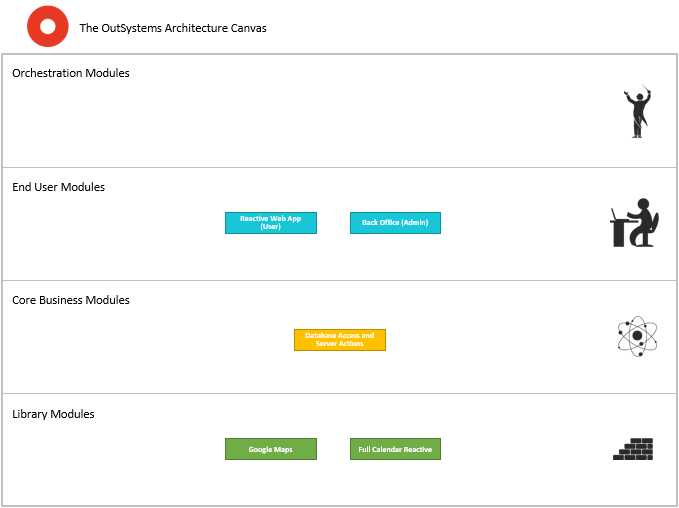
\includegraphics[scale=0.7]{figures/4LayerCanvas.png}
  \caption{4 \textit{Layer Canvas}}\label{fig:4lc}
\end{figure}

Esta metodologia propõe que se estruture as várias funcionalidades da aplicação por quatro camadas, sendo estas, começando por baixo: 

\begin{itemize}
    \item \textit{Library Layer} --- Aqui devem constar os módulos que são transversais ao domínio do problema, tais como: temas, bibliotecas, etc. 
    \item \textit{Core Layer} --- Módulos referentes à lógica de negócio, modelo de dados e \textit{server actions}. 
    \item \textit{End User Layer} --- Nesta camada é tratada toda a parte de interface e experiência do utilizador, fazendo uso das camadas anteriores. 
    \item \textit{Orchestration Layer} --- Camada que coordena a comunicação entre várias aplicações. 
\end{itemize}

É importante verificar que, apesar da metodologia apresentar quatro camadas, 
a nossa arquitetura apenas faz uso das primeiras três devido ao nosso projeto consistir em apenas uma aplicação reactive, 
e não havendo necessidade de coordenar interações com outras aplicações na camada de orquestração. 
Posto isto, a nossa aplicação assenta sobre cinco módulos, representados pela figura~\ref{fig:4lc}.

Começando pela \textit{Library Layer} verificamos que são utilizados os módulos relativos à integração da aplicação 
com o \textit{Google Maps} e com o \textit{Full Calendar Reactive}. De seguida temos a \textit{ Core Layer}, 
onde definimos as entidades de domínio e suas operações. Por fim a \textit{ End User Layer} onde são definidos 
os ecrãs e a lógica de cliente. 

\begin{figure}[H]
  \centering 
  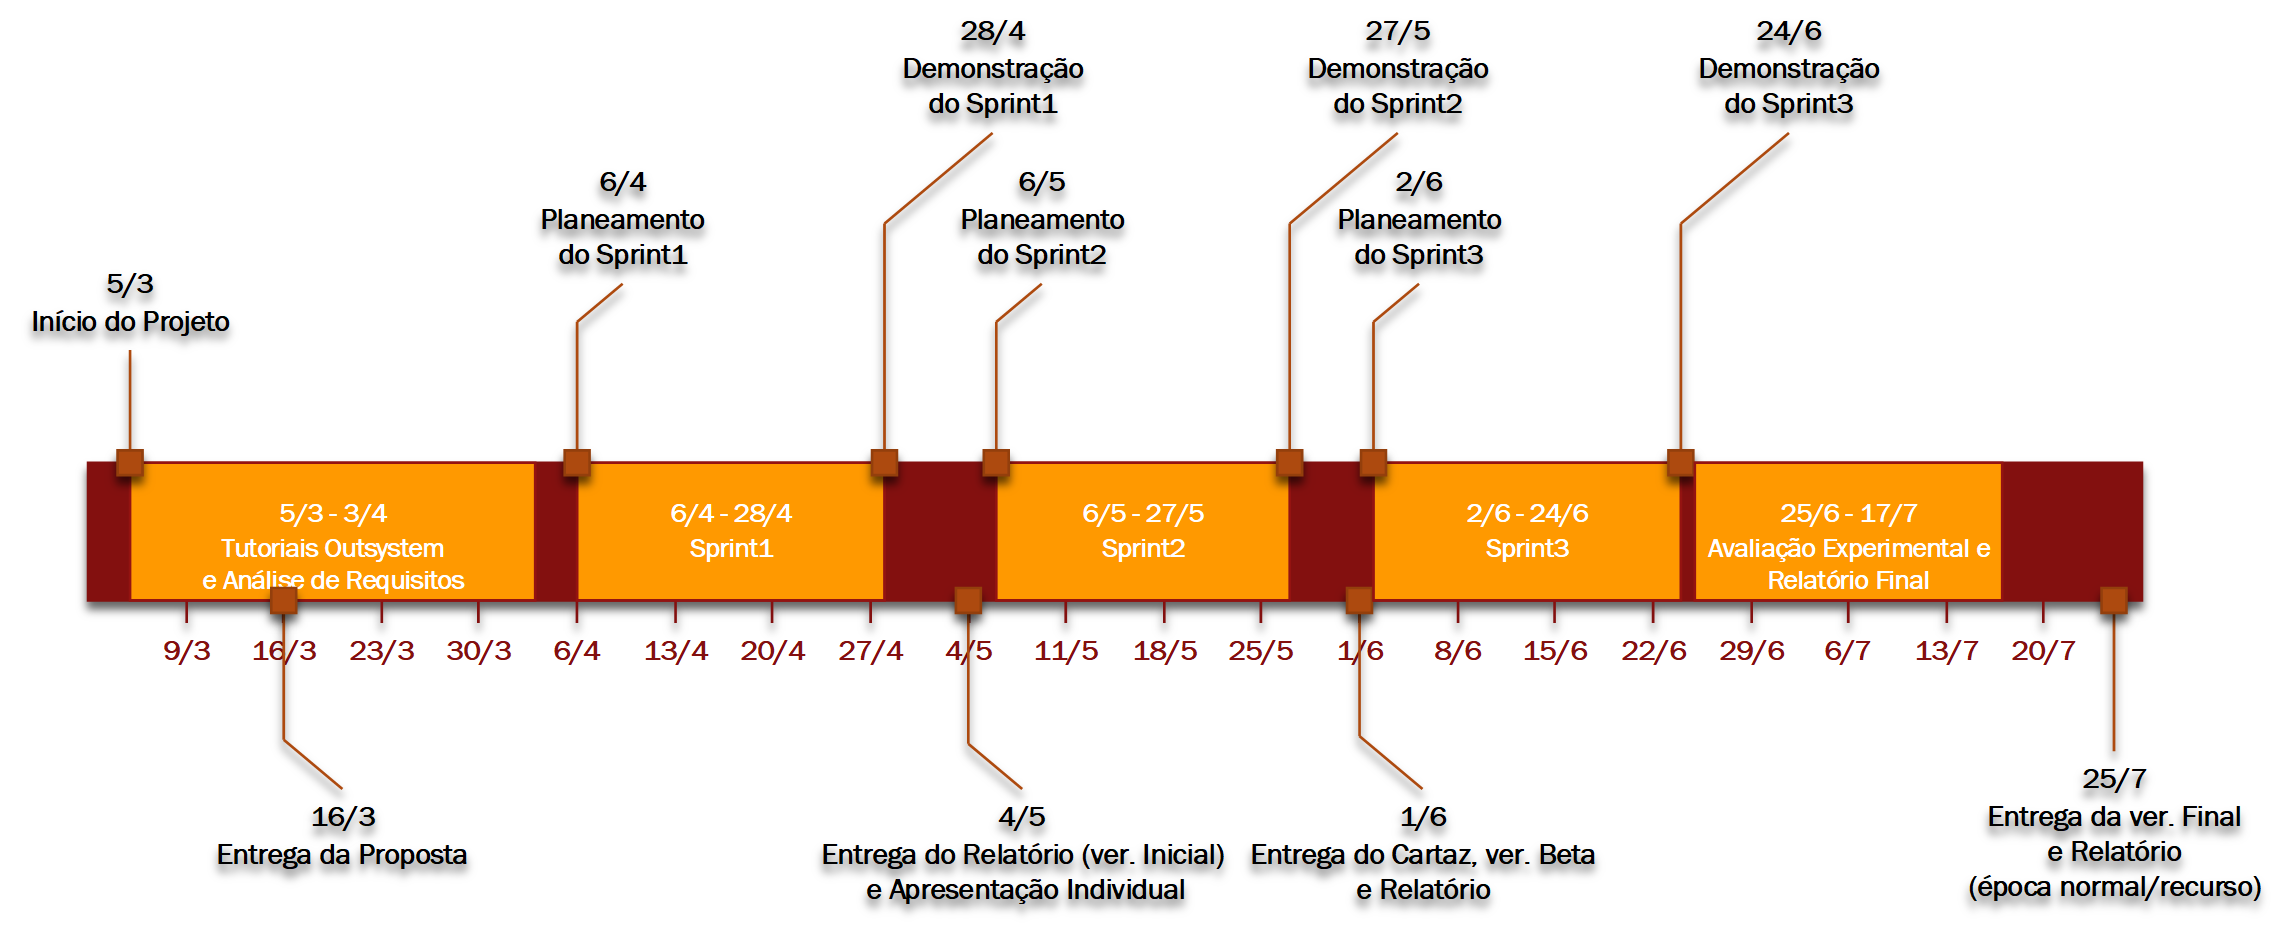
\includegraphics[scale=0.4]{figures/Timeline.png}
  \caption{Timeline}\label{fig:timeline}
\end{figure}

\addcontentsline{toc}{section}{Conclusão}
\section*{Conclusão}\label{sec:conclusion}

De uma forma geral, o progresso do projeto está de acordo com o planeamento apresentado anteriormente, na proposta de projeto, e novamente, na figura~\ref{fig:timeline}.

Inicialmente, devido à pesquisa e aprendizagem de algumas tecnologias novas, o desenvolvimento ocorreu de forma mais lenta. 
No entanto, após ultrapassado esse obstáculo, o ritmo de trabalho aumentou de forma considerável e consequentemente os resultados surgiram também mais rapidamente. 

De momento, a aplicação já possui um modelo de dados estruturado e algumas funcionalidades, nomeadamente a possibilidade de criação, 
inscrição e visualização de uma necessidade, e um \textit{back office} que permite adicionar e/ou remover categorias possíveis de uma necessidade. 
Para além disto, foi desenvolvida uma outra funcionalidade que estava no planeamento ser realizada no próximo sprint, nomeadamente a visualização das necessidades dispostas num calendário.
\end{document}